\chapter{Implementation}

\section{Hardware platform}
In this section, a detailed explanation of the choices regarding hardware components, communication protocols and software, is provided.\\

The hardware platform is implemented on a Printed Circuit Board (PCB). An overview of the components used is provided in \cref{fig:hardware_overview}. The schematics and the PCB layout is included in \cref{sec:pcb}.\\
The hardware platform is powered by USB which runs on 5V. The electronic circuit contains 2 microcontrollers \textit{ESP-12E} and \textit{ATmega32u4}. ESP-12E is selected because of the necessity of a WiFi connection between the hardware and GUI. This topic is explained in detail in \cref{sec:conn_with_GUI}. ATmega32u4 provides the USB-MIDI interface. This interface is explained in \cref{sec:usbinterface}.\\
ESP-12E runs on 3.3V therefore a linear voltage regulator was added to the circuit. The 2 microcontrollers communicate using I2C (Inter-Integrated Circuit) but their supply voltages are different. A logic level shifter is added to convert 3.3V logic to 5V logic.
Due to the large number of digital inputs from the keypad and the rotary encoders, shift registers are needed to serialize the data and pass it to the ATmega microcontroller.

\begin{figure}[H]
    \centering
    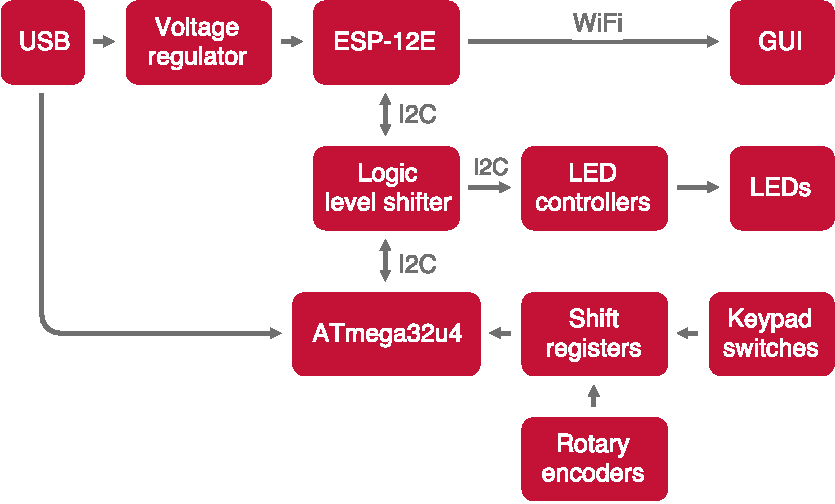
\includegraphics[width=0.7\textwidth]{graphics/hardware_overview.pdf}
    \caption{Overview of the hardware platform}
    \label{fig:hardware_overview}
\end{figure}


\subsection{USB interface}
\label{sec:usbinterface}
The USB-MIDI interface falls under the Human Interface Device (HID) class, which describes devices such as mouse devices, keyboards, gaming controllers etc., that all follow a strictly described and standardized protocol. Devices within the HID class features self describing messages, for initializing communication with a dedicated HID driver on a computer. The driver parses the data, enabling generic software applications to use the data directly.\cite{HID} \\
For this project, the USB-MIDI interface therefore allows the platform to communicate with all DAW's that support MIDI, without a specialized driver or other middleware, which is preferred in terms of accessibility.\\

For a device to apply with the USB-HID specification, it must feature an USB-controller, a chip that implements the low level USB protocol, by maintaining the USB peripherals D+ and D-.\\ 
It prepares and encodes data for transmission, buffers and decodes received data, and provides connection detection as well as error indication.\\
Dedicated USB-controller chips isn't used as widely anymore, as many microcontrollers come with built in USB peripherals, allowing higher speed and easier interaction. 

In this project the \textit{ATmega32U4} microcontroller is used, as it is a low cost IC, standard in many embedded applications and features a USB-controller. \\
It operates at 16 MHz, has 16K bytes on-chip flash memory, and a 10-bit high speed counter, making it usable for other purposes than simply forwarding MIDI to USB, see \cref{sec:UI}.
Furthermore the ATmega32U4 is a part of the ATMEL AVR family, and is therefore compatible with Arduino libraries. It is in fact used in the open source platform "Pro Micro" by \textit{Sparkfun}, and their circuitry of external components is used "as is" in this project, see \cref{app:micro}.

\subsection{Communication between GUI and harware}
\label{sec:conn_with_GUI}
In order to establish connection between the hardware platform and the GUI different technologies was surveyed. As the hardware platform already included a USB interface this was the first solution considered. The USB interface had several drawbacks though. First of all MIDI was considered a too limited form of communication for the purpose of sending data back and forth between the GUI and the hardware platform. If the standard was exceeded it would require a custom driver for each platform. Second the USB interface is implemented as having only one host which is not convenient if a user wants to use the GUI on both a computer and a phone on the same time. It was found that network would be a better solution for this and as Ethernet is not available on many laptops and not available on any phones and tablets,  WiFi was selected as the appropriate technology.

\subsubsection{Embedded WiFi technologies}

To embed WiFi into the hardware platform 3 SoCs (System on a Chip) were considered: \textit{ESP8266}, \textit{Raspberry Pi Zero W} and \textit{C.H.I.P. Pro}. We selected these as they are easy to use and have a large community. These are listed in \cref{tab:wifi} with the relevant attributes for the platform.\\
As the CPU and memory requirements for this application are quite low, the most relevant differences between the 3 SoCs is cost and operating system. Both \textit{C.H.I.P. Pro} and \textit{Raspberry Pi Zero W} are single board computers running Linux which has a lot of advantages as Linux ships with lots of tools for code debugging and maintenance. The disadvantage is that Linux is a general purpose operating system which makes precise low-level hardware interfacing more difficult.\\
The \textit{ESP8266} is a SoC developed by \textit{Espressif Systems} as is available as a WiFi module with antenna as \textsc{ESP-12E}. The ESP8266 has no operating system but supports the \textsc{Arduino}-environment which makes firmware development very easy. As low cost and low-level hardware interfacing are significant requirements for the hardware platform the ESP12-E was chosen as the WiFi module.

\begin{table}[h]
    \centering
    \begin{tabular}{c c c c c c}
        & \thead{Operating\\system} & \thead{Clock\\frequency} & \thead{Power usage [W]} & \thead{Storage} & \thead{Cost [USD]} \\
        ESP8266 (ESP-12E) & None & 80 MHz & 0.56 \cite{website:esppower} & 4 MB flash & 1.94\\
        Raspberry Pi Zero W & Linux & 1 GHz & 0.85 \cite{website:rasppower} & SD-card & 10\\
        C.H.I.P. Pro & Linux & 1 GHz & - & 512 MB flash & 16
    \end{tabular}
    \caption{Comparison of easy-to-use embedded WiFi SoCs (System on a Chip)}
    \label{tab:wifi}
\end{table}


\subsection{LED controller}

The user hardware platform contains 48 LEDs: 24 red and 24 green. These are all placed under the rubber keypad buttons. It is stated in \cref{sec:UI} that the LEDs should be dimmable. To implement this the \textit{TLC59116} LED controller is chosen. It is suited for to this application for several reasons. First it uses the I2C protocol to interface with the microcontroller. This is already implemented to communicate between the microcontrollers on the board. Second it is able to drive 16 LEDs at a time, which means that only 3 instances of the component is needed. Finally it is able to drive each LED without a series resistor, which saves 48 resistors from the bill of materials. The LED controller is controlled by the ESP8266 which uses the Arduino library TLC59116 to set the brightness of each LED.
 
\section{Microcontroller firmware}

The firmware for the hardware platform consists of two layers the \textit{application layer} and the \textit{hardware abstraction layer}. An overview of the modules contained in the firmware is seen in \cref{fig:firmware}. The application layer implements the sequencing part of the platform. 
This layer is a part of the program \textsc{torso\_esp} and runs on ESP8266. This is chosen because ESP8266 has higher performance than ATmega32u4 and supports the \textit{Standard Template Library}, which contains many handy abstractions. The application layer is designed to be platform independent, which makes the code compatible with both ESP8266 and x86-64 architecture. This enables the application layer of the firmware to be tested on a PC. This approach shortens the firmware development as the process of compiling and uploading to ESP8266 using Arduino IDE is very slow.

The \textit{hardware abstraction layer} is split into two programs \textsc{torso\_esp} and \textsc{torso\_atmega}. This layer implements handling of inputs from rotary encoders and buttons, communication with the GUI and output through MIDI.


\begin{figure}[h]
    \centering
    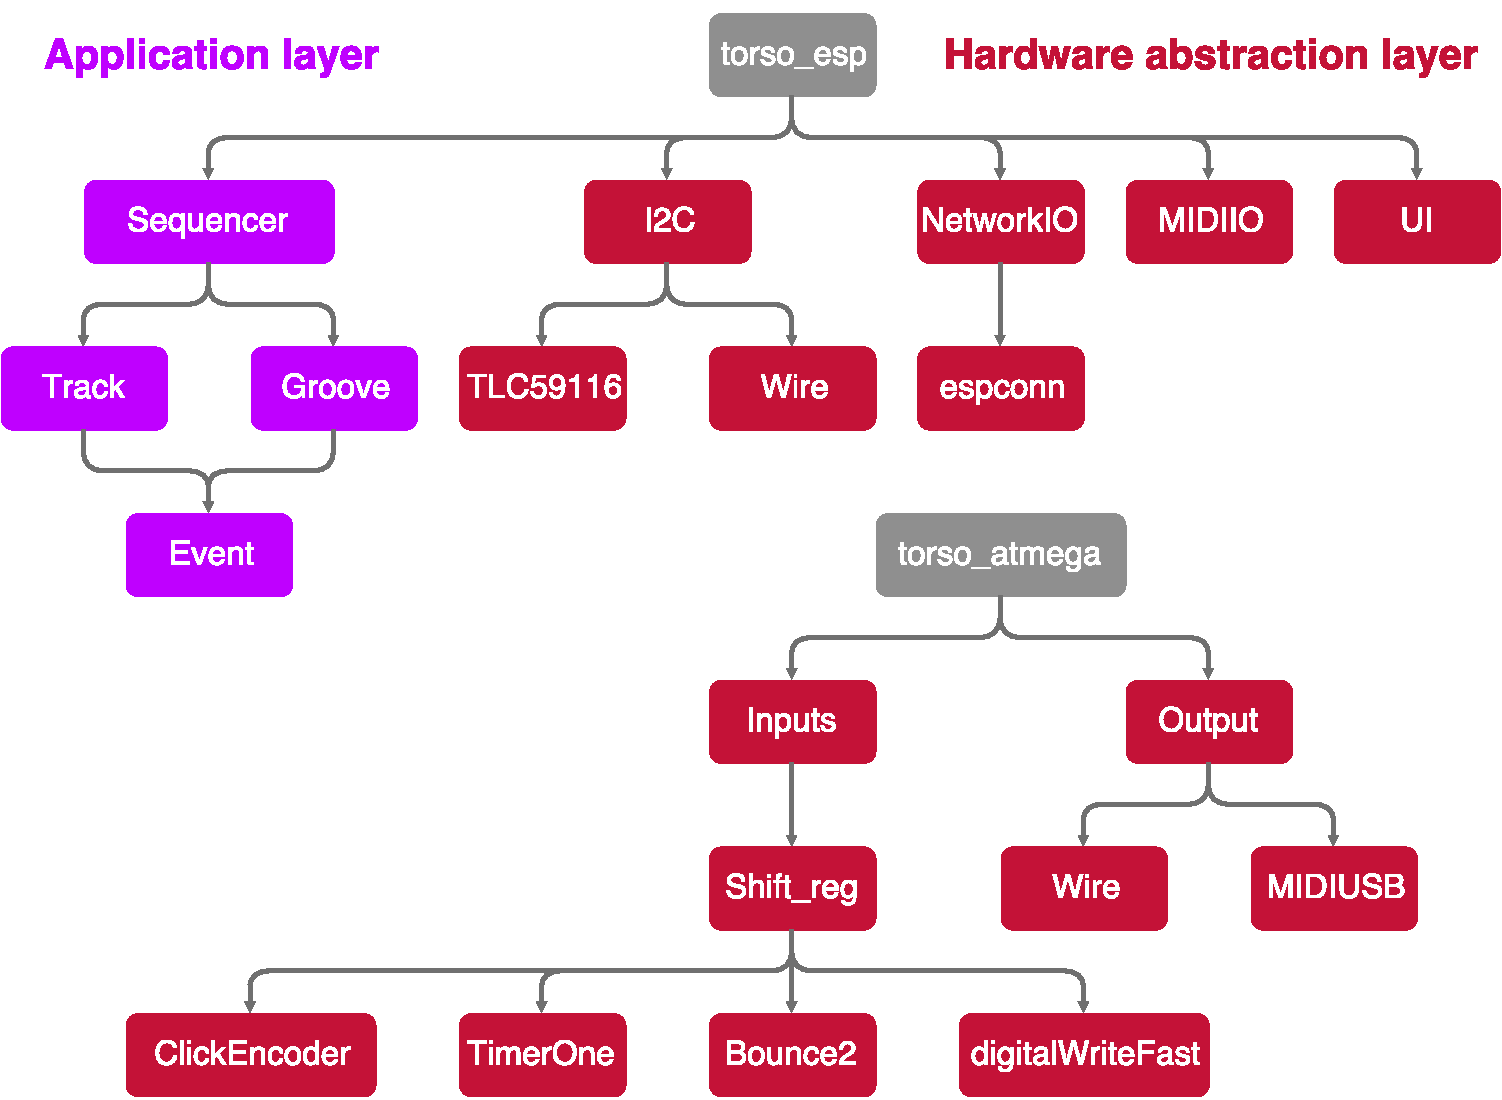
\includegraphics[width=\textwidth]{graphics/firmware_overview.pdf}
    \caption{Class hierarchy of firmware \tdr{caption class hierarchy}}
    \label{fig:firmware}
\end{figure}

\subsection{Hardware abstraction layer}
\label{sec:harwarelayer}

\subsubsection{User interface I/O}
\label{sec:userinterfaceio}
The parallel to serial converter \textsc{74HC165} is used to serialize the parallel inputs and read them into ATmega32u4. The flowchart for the shift-in routine is seen in \cref{fig:atmegaflow}. The serial data split into two parts, one for the buttons and one for the rotary encoders. The data for the buttons is debounced using the Arduino library \textsc{Bounce2} and saved into a binary array. The data for the encoders saved into an array of the class \textsc{ClickEncoder}, which is a modified version of the Arduino library with the same name. This class implements a state machine to handle the 2-bit gray code produced by the rotary encoders. This encoding consists of to PWM-signals, with a relative phase difference as a measure for the turning direction. Reading the phase shift accurately requires a high and precise clock rate, and the shift in routine is therefore clocked by an on-board hardware timer, with a period of  $\SI{20}{\micro\second}$.

\begin{figure}[H]
    \centering
    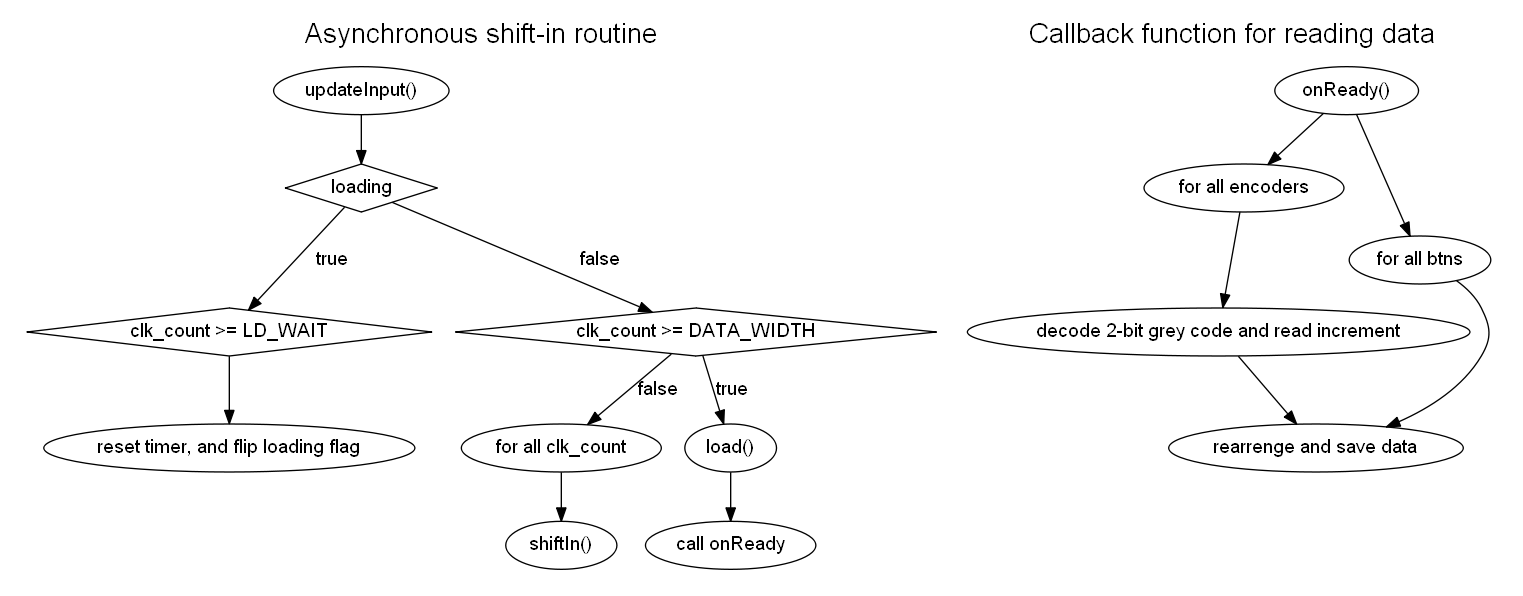
\includegraphics[width=\textwidth]{graphics/atmega_flow.png}
    \caption{10 parallel to serial converters \textsc{74HC165} is used to read inputs from 18 rotary encoders and 24 buttons. Each contains 8 registers that hold 8 bits of data, and by clocking the registers, the data is shifted in serially. This is managed by the function \textit{shiftin()}. When all data is shifted in, the load pin is pulled low, to load in new data to the registers. This is managed by \textit{load(}). The callback function \textit{onReady} manages the preparation of the raw data, including decoding the encoder signal to a direction (-1,0,1)
    }
    \label{fig:atmegaflow}
\end{figure}

When the ESP12-E request for the user interface the relative increment of the rotary encoders and the binary value of the buttons are encoded into a byte array and transmitted to the ESP12-E. A flowchart for this routine is seen in \cref{fig:i2c}.

\begin{figure}[H]
    \centering
    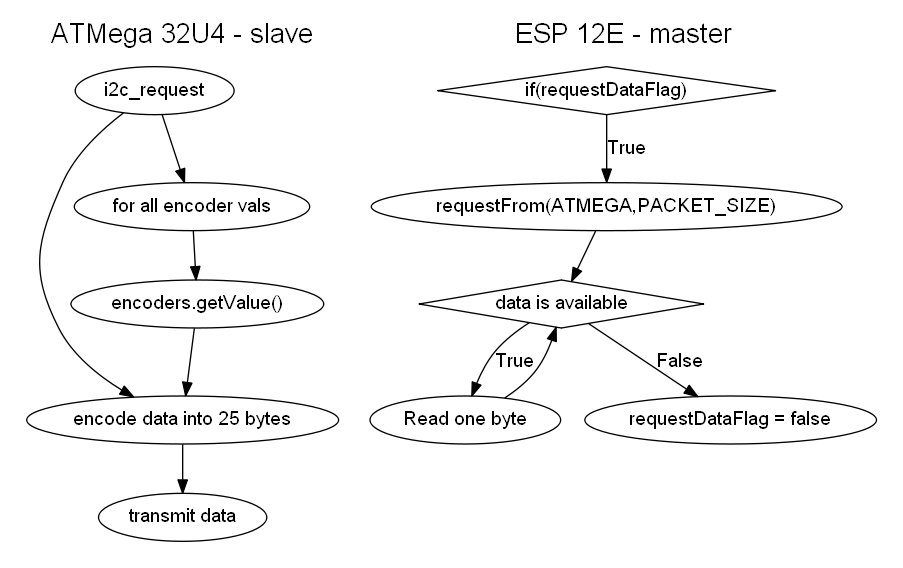
\includegraphics[width=0.7\textwidth]{graphics/i2c_flow.png}
    \caption{Flowchart for I2C communication between microcontrollers \tdr{caption}}
    \label{fig:i2c}
\end{figure}

\subsubsection{Network}
\label{sec:networkconf}

The connection between GUI and the hardware platform is implemented using WiFi (see \cref{sec:conn_with_GUI}). To achieve transmission of data through WiFi the transport layer of the Internet prototol suite (TCP/IP) is needed. The main protocols within the transport layer are called Transmission Control Protocol (TCP) and User Datagram Protocol (UDP). The decision on which one to use is a trade-off between efficiency and reliability where TCP is generally more reliable but also slower than UDP\cite{website:tcpvsudp}. When it comes to the GUI, responsiveness rather than reliability is preferred therefore UDP was selected as the appropriate protocol.

Before data can be transmitted between the ESP8266 WiFi module and the device running the GUI, the two has to be on the same network. The ESP8266 has two WiFi configurations: \textit{STA} (Station mode) and \textit{SoftAP} (Software enabled access point mode). STA-mode enables the ESP8266 to connect to a WiFi router given a SSID (Service set identifier) and a password. SoftAP-mode enables the ESP8266 to create a WiFi access point which other devices can connect to. As the WiFi connection on the device running the GUI is most often already in use for other purposes such as accessing the internet, STA-mode is more practical as the user can connect to the ESP8266 through his/hers own router. STA-mode has the disadvantage though that it needs a configuration interface through a wired connection as the user needs to supply the SSID and password for his/hers home network. With SoftAP-mode the SSID and password can be fixed and supplied with the platform. Although this solution has potential security issues this configuration was chosen as the development of a WiFi configuration interface was considered outside of the scope of this project.

Three libraries for working with network on ESP8266 was tested:
\begin{itemize}
    \item ESP8266WiFi Arduino library
    \item lwIP (lightweight IP)
    \item Espressif Non-OS SDK
\end{itemize}
The \textit{ESP8266WiFi} is easy to set up and use but after thorough testing it was found that with a seemingly random interval the transmission of UDP would hang for 1-2 seconds. By exploring the source code of the library it was found that 
ESP8266WiFi depends on \textit{lwIP}, an open source TCP/IP stack designed for embedded systems. When trying to use lwIP directly the same pattern was observed and it was thus concluded that the problem had to reside within the lwIP implementation for ESP8266. After an unsuccessful search for others having the same problems the lwIP library was discarded.

Later it was found that \textit{Espressif} (the maker of ESP8266) had created a SDK for ESP8266 which included a module \textit{espconn} for working with WiFi. The system was tested using this module instead and the transmission was suddenly a lot more reliable. No traces of the pattern described above was found after changing from lwIP to espconn.

% The network module of the ESP8266 firmware has to two functions: \textsc{NetworkIO::init} and \textsc{NetworkIO::sendPacket}.

% \textsc{NetworkIO::init} is called from the top-level initialization function and creates the WiFi access point and initializes the UDP connection. A fixed IP address is automatically assigned to the first device connecting to the access point.

% \textsc{NetworkIO::sendPacket} takes a pointer to an array of bytes and the size of the array as arguments and transmits the data to the fixed IP address. This allows only one device running the GUI to be connected at a time.

% The \textsc{Sequencer} module calls \textsc{NetworkIO::sendPacket} in two cases. 

% \tdr{skriv færdig}

\subsection{Application layer}
\label{sec:applicationlayer}

The application layer implements all functionality related to the sequencing part of the hardware platform. This layer is designed to be platform independent. An overview of the API used is provided in \cref{fig:torsoapi}.

\begin{figure}[H]
    \centering
    \begin{factbox}
        \textbf{Sequencer} contains an array of   \textbf{Track}s. Does scheduling of all \textbf{Event}s.
        \\\\
        \textbf{Track} represents a rhythm. The rhythm is defined by a binary sequence generated using Bjorklund's algorithm (see \cref{sec:bjorklund}). Also contains all parameters described in \cref{tab:params}. Generates \textbf{Event}s.
        \\\\
        \textbf{Event} represents a rhythmic event. It is a \textsc{struct} that has the fields \textbf{position} and \textbf{time stamp} along with MIDI parameters such as \textbf{pitch}, \textbf{velocity} and \textbf{type} (Note on/off and rest).
        \\\\
        \textbf{position} is a floating point number describing the distance to the beginning of the binary rhythm sequence. The distance is given in the unit of steps.
        \\\\
        \textbf{time stamp} is the scheduled absolute time in microseconds for an \textbf{Event}.
        \\\\
        \textbf{Groove} represents a fixed rhythm. The rhythm is defined by an array of \textbf{Event}s.
    \end{factbox}
    \caption{Overview of the application layer API}
    \label{fig:torsoapi}
\end{figure}

\subsubsection{Sequencer}
\label{sec:sequencer}
The core of the \textsc{Sequencer} module is the \textsc{update} function which is visualized as a flowchart in \cref{fig:sequencer}. This function is called in the main loop of the top module. A key element in \textsc{Sequencer} is the \textsc{eventQueue}, which is a priority queue that contains all events scheduled. The priority queue data structure ensures that the events will be scheduled at the right time and in correct order according to the time stamp of the events.
Timekeeping on the ESP12-E is based on the Non-OS SDK function \textsc{system\_get\_time()} which returns the time in microseconds since the system turned on. When time exceeds the time stamp of the event in the front of \textsc{eventQueue} the MIDI data of the event is transmitted to ATmega32u4 through I2C. When the ATmega32u4 receives the data it is simply forwarded through the USB interface using the Arduino library \textit{MIDIUSB}.\\ 
As basis for calculating time stamps the variable \textsc{stepTime} is used. \textsc{stepTime} is defined as the interval in microseconds between each step in the rhythm generated by the euclidean algorithm. \textsc{stepTime} is calculated from commonly used musical timing parameters:
\begin{equation}\label{eq:steptimecalc}
\text{stepTime} [\SI{}{\micro\second}] = 10^6 \times
\left(\frac{
\text{tempo} [\SI[per-mode=fraction]{}{\beats\per\minute}]
}{
60
}\right)^{-1}
\times
\SI{4}{\beats} \times \text{division}    
\end{equation}

where \textsc{tempo} is defined as beats per minute and \textsc{division} as the note value of a note in a bar with 4 beats. In order to reduce the jitter of the animation in the GUI (see \cref{sec:guiimplementation}) a buffer of 4 steps is calculated at a time. The \textsc{bufferLength} (length of buffer in microseconds) is calculated as

$$
\text{bufferLength} = 4 \times \text{stepTime}
$$

When the user starts the sequencer the current time is saved as \textsc{timeOffset}. When time passes by $\textsc{bufferLength} + \textsc{timeOffset}$ a new \textsc{timeOffset} is saved and the \textsc{calculate} function on each \textsc{Track} is called. This function is visualized as a flowchart in \cref{fig:calculate}.

\begin{figure}[H]
    \centering
    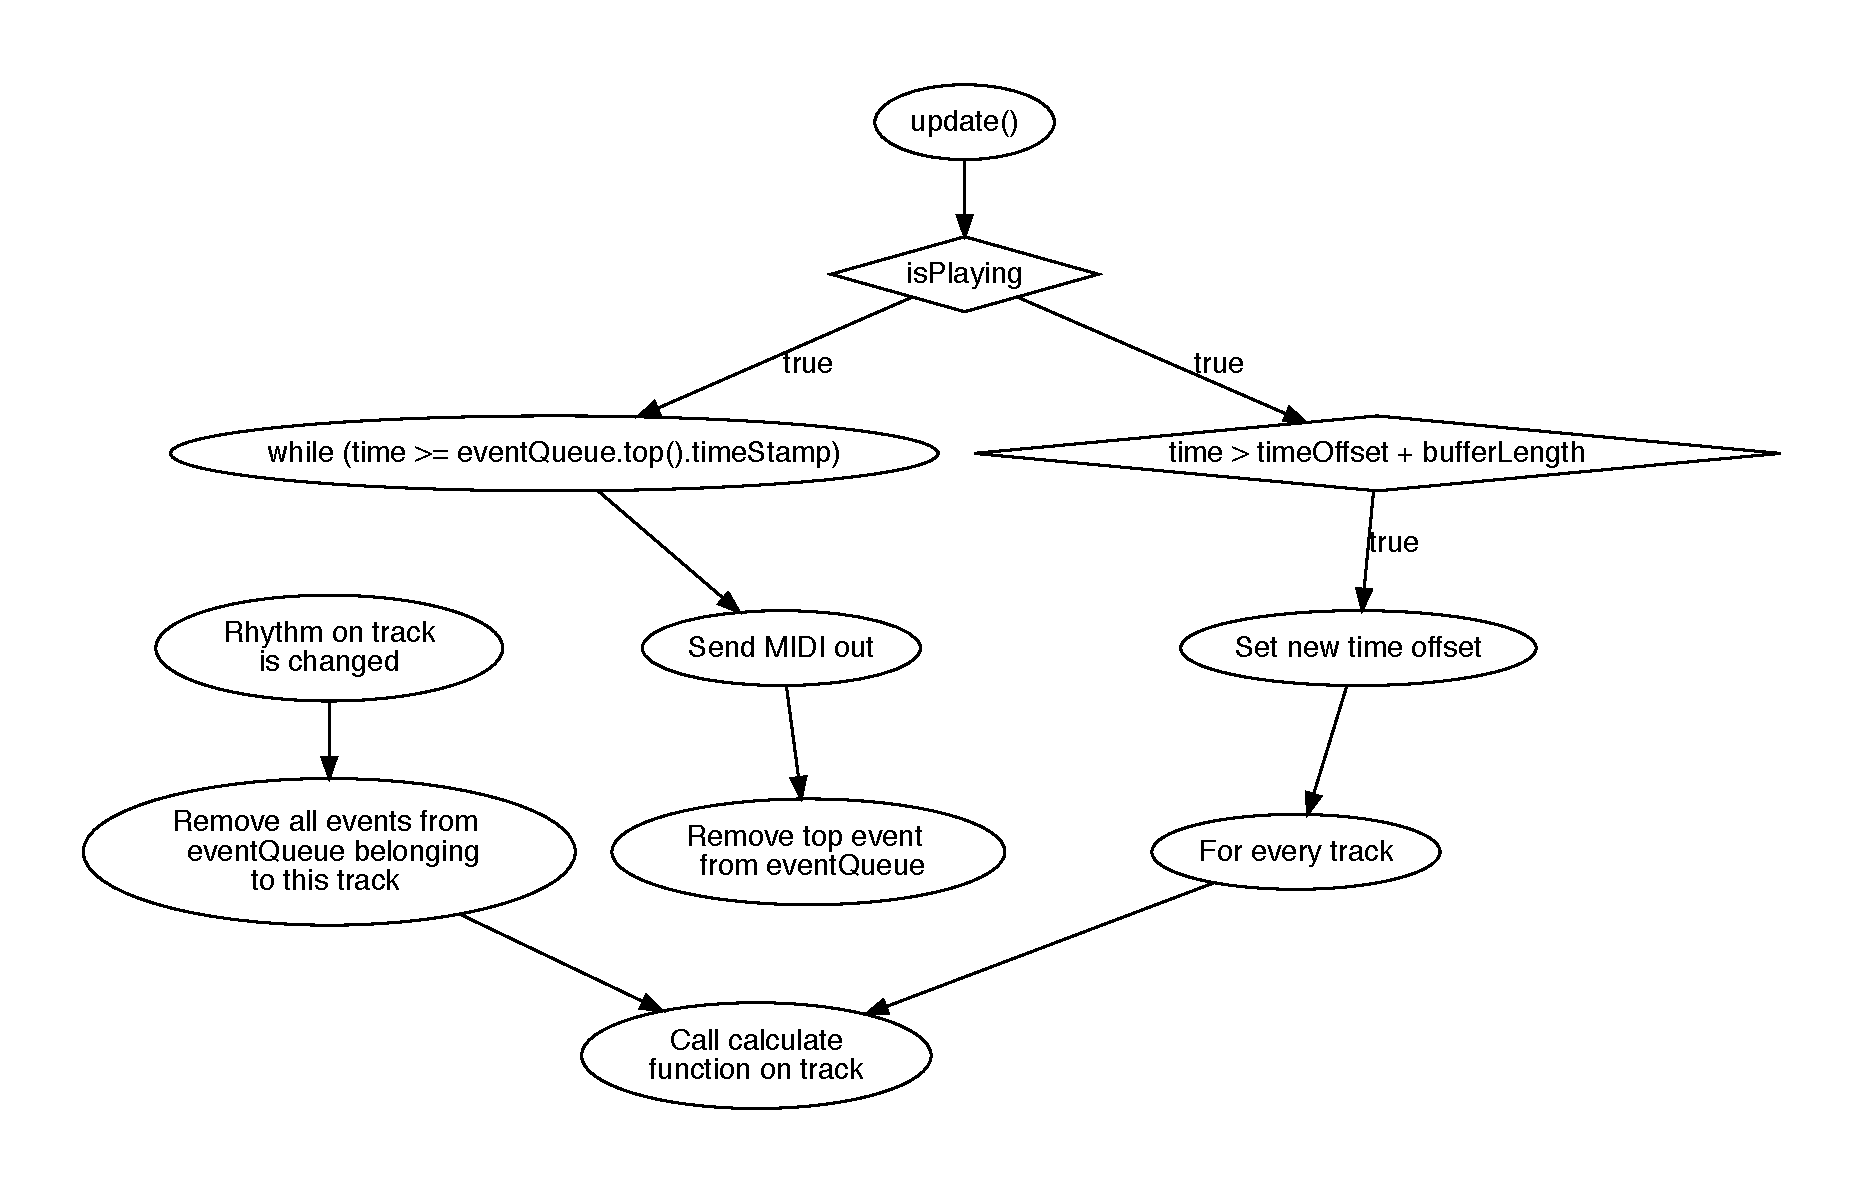
\includegraphics[width=\textwidth]{graphics/sequencer.pdf}
    \caption{Flowchart of the \textsc{Sequencer::update} function. \tdr{caption sequencer update}}
    \label{fig:sequencer}
\end{figure}

\begin{figure}[H]
    \centering
    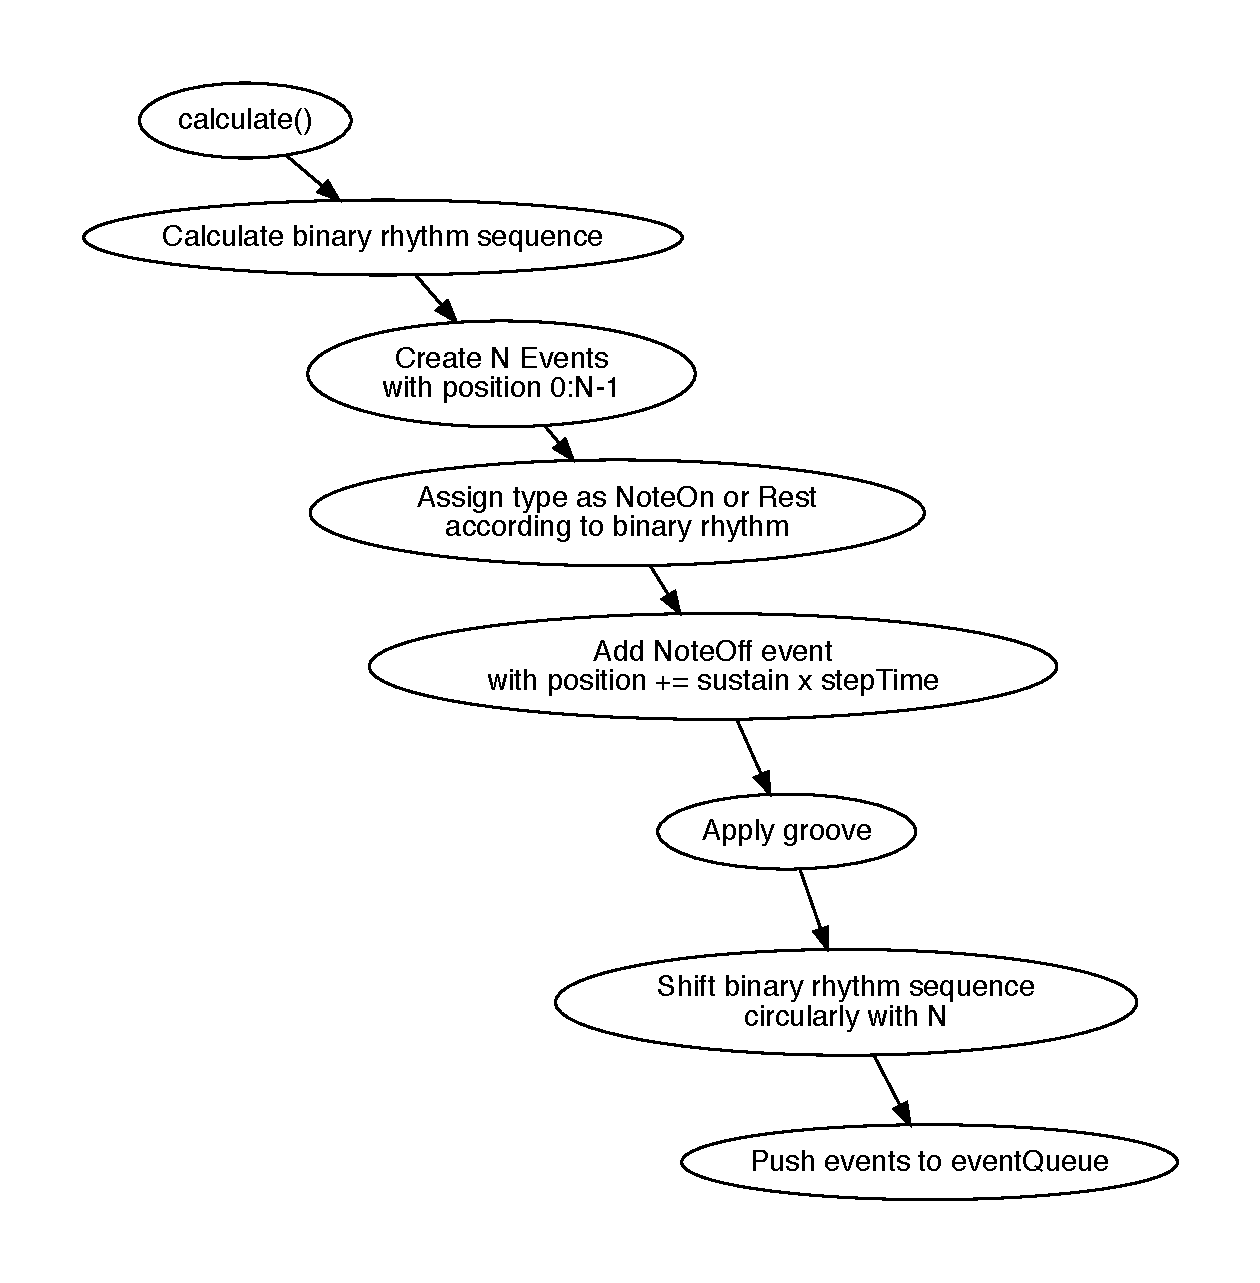
\includegraphics[width=0.7\textwidth]{graphics/calculate.pdf}
    \caption{Flowchart of the \textsc{Track::calculate} function. $N$ refers to the number of \textsc{Event}s in the buffer. The calculation of the binary rhythm sequence is implemented as described in \cite{bjorklund}. As an optimization this step is only carried out if steps, pulses or offset has changed. The event type is assigned to \textsc{NoteOn} for all 1's and \textsc{Rest} for all 0's in the binary sequence. \textsc{sustain} is a number between 0-1 giving a maximum sustain of 1 step. The "Apply groove" step is written as pseudo code in \cref{lst:groove}}
    \label{fig:calculate}
\end{figure}

The groove system used in the "Apply groove" step in \cref{fig:calculate} is implemented using the \textsc{Groove} class. This class represents a groove as a vector of \textsc{Event}s. The \textsc{Groove} class has a member function \textsc{getNearestEvent} which takes an integer as argument. The function returns the event which has a unit time stamp closest to the input argument. When the nearest event is found the interpolation described in \cref{sec:groovesystem} is carried out. The pseudo code of the implementation is seen in \cref{lst:groove}.

\begin{lstlisting}[caption={Pseudo code of "Apply groove" step \tdr{caption}},label={lst:groove},float,floatplacement=H]
applyGroove():
    for e in events:
        e´ = getNearestEvent(e)
        e.pos = interp ( e.pos, e´.pos, timing * grooveAmount )
        e.pos += rand(-1, 1) * randomTiming * grooveAmount
        e.vel = interp ( e.vel, e´.vel, grooveVelocity * grooveAmount )
        e.vel = interp ( e.vel, rand(0,127), randomTiming * grooveAmount )
        e.timeStamp = timeOffset + e.pos * stepTime
        
    circshift(groove, length(events))
\end{lstlisting}

% \begin{figure}[h]
%     \centering
%     \includegraphics[width=\textwidth]{graphics/groove.pdf}
%     \caption{Flowchart of the "Apply groove"-step in \cref{fig:calculate}. All the interpolation factors (\textsc{timing}, \textsc{grooveVelocity} and \textsc{randomTiming} are scaled by \textsc{grooveAmount}}
%     \label{fig:groove}
% \end{figure}

\section{GUI} % Presentation layer
\label{sec:guiimplementation}

In order to implement the GUI, a GUI library is needed. Different libraries fulfilling the following specifications were surveyed.

\begin{itemize}
    \item In order to make the platform accessible to as many as possible the GUI is required to be cross-platform i.e. the GUI should be able to run on iOS, Android, macOS, Windows and Linux.
    \item The GUI should support network sockets to connect with the hardware platform.
    \item The GUI should have high runtime performance as responsiveness is important in musical context. 
\end{itemize}

3 GUI technologies were found that met the requirements above: \texttt{HTML5}, \texttt{Qt} and \texttt{JUCE}. A comparison of these is seen in \cref{tab:GUI}. \textit{HTML5} differs from the others by not being a GUI library but rather referring to modern web technology using the newest features of JavaScript. Code written in JavaScript is differs from code written in C++ by not being native. While code written with both Qt and  JUCE is compiled into machine code before being available to the user. Code written in JavaScript is compiled at runtime. This makes HTML5 significantly slower than the others in general. Though the development time of HTML5 apps is shorter than in C++ it was deemed that the HTML5 would not perform well enough for a music app. Also HTML5 only provides \textit{WebSockets} (a TCP based protocol but with a much larger overhead than UDP) for network transmission.\\
Therefore HTML5 was discarded as an option. An important difference between Qt and JUCE is that JUCE is developed by \textit{ROLI} a music hardware company so JUCE comes with a lot of components meant for music apps. Therefore JUCE was chosen as the GUI library.

\begin{table}[H]
\centering
\begin{tabular}{ l c c c }
&

\includegraphics[height=0.1\textwidth]{graphics/html5.png} &

\includegraphics[height=0.1\textwidth]{graphics/qt.png} &

\includegraphics[height=0.1\textwidth]{graphics/juce.png} \\
Language            & JavaScript & $\text{C++}^*$ & C++ \\
Sockets             & Websockets only & Yes & Yes\\
Native & No & Yes & Yes \\
\end{tabular}
\caption{Comparison of cross-platform GUI technologies.}
\label{tab:GUI}
\end{table}

The GUI has two components \textsc{SequencerComponent} and \textsc{NetworkIO}. The \textsc{SequencerComponent} implements the user interface using the \textsc{Graphics} class from the JUCE library. This class has member functions to draw geometric primitives such as rectangles, circles, lines etc. The actual drawing of primitives is done by overriding the \textsc{paint} function of \textsc{SequencerComponent}. In this functiontThe graphical representation of the euclidean rhythm was implemented.\\
The \textsc{NetworkIO} component implements the communication with the hardware platform. This is done by creating a thread that waits for incoming UDP messages. The UDP messages included the value of all the rhythmic parameters. Additionally the UDP messages included the variable \textsc{activeStep} to indicate the progression in the euclidean rhythm. The initial implementation 
is described in following:
Every time a UDP message is received the function \textsc{repaint} of \textsc{SequencerComponent} is called, which redraws the graphical representation of the euclidean rhythm. The \textsc{activeStep} is visualized by increasing the size of the circle as seen in \cref{fig:app}.\\
As the WiFi connection suffered from significant variable latency the animation was very jittery. Therefore the implementation was changed. First the core of the sequencer firmware was copied into the app. Then a buffer with the size of 4 events was introduced into the sequencer firmware. Every time a new buffer with events is calculated it is sent to the app. By using the time stamp information of the events in the buffer both the app and firmware were able to trigger the events at the correct time. This solution removed much of the jitter in the animation.

        % 

% LOG - summarize

    % PCB 
    
        % Choice of encoders 
        % issues
            % Voltage drop when usb powered
            % datasignal q1 shorted to 5v.
            % Pull up resistors
            % Wrong pins ( no suitable alternate functions) for shift registers
                % Use PB5 for SHIFT_CLK_PIN - pin change interrupt
                % Use PB6 for SHIFT_DATA_PIN, output conmpare or pwm from timer1, to make steady clock
                    % Wire clock enable from all 74HC165 to general purpose I/O pin on atmega or use enable register
            
    
    % ATMEGA
        % USB MIDI
        % Encoder
            % Wrong pins
            % Debounce on all inputs - debounce on only buttons
            % DigitalWritefast
    % APP
    % ESP prgramming
        % implement basic scheduler
            % event data type, timestamp, priority queue
            % tracks
            % calculate function
                % euclid calculation
                % state saving
                % snap to groove
                % groove forward calculation
                
            % 
        % from softwaretimer to  millis()
        